\documentclass[a4paper,zihao=-4,AutoFakeBold]{ctexart}

\usepackage[top=2.5cm,bottom=2.5cm,left=2.8cm,right=2.8cm]{geometry}
\usepackage{fontspec}
% 使用类 Times 西文字体
\setmainfont{texgyretermes}[
    Extension      = .otf ,
    UprightFont    = *-regular,
    BoldFont       = *-bold,
    ItalicFont     = *-italic,
    BoldItalicFont = *-bolditalic,
]
% 你也可以把上面的字体设置命令去掉,改为下面的 Times New Roman
% \setmainfont{Times New Roman}
\usepackage{amsmath}
\usepackage{amssymb}
\usepackage{color}
\usepackage{graphicx}
\usepackage{tabularx}
\usepackage{enumitem}
\usepackage{array}
\usepackage{makecell}
% 可使用 style=gb7714-2015 选项来指定参考文献国标样式,但官方模板对此未做要求
% 使用 sorting=none 选项指定按照文章内引用顺序来排序参考文献
\usepackage[maxbibnames=9,sorting=none]{biblatex} 
\addbibresource{ref.bib}
\usepackage{etoolbox}
\usepackage[hidelinks]{hyperref}

\newcommand{\Tr}{\operatorname{Tr}_1^n}
\newcommand{\F}{\mathbb{F}}
\newcommand{\Fn}{\mathbb{F}_{2^n}}
\newcommand{\R}{\mathbb{R}}
\newcommand{\Z}{\mathbb{Z}}



% 绘制 ``研究课题来源'' 表格里用到的勾和框
% \myunchecked 绘制未打勾的方框
% 定义 ``研究课题来源'' 表格里用到的勾和框
\xeCJKDeclareCharClass{CJK}{"25A1}
\newcommand{\myunchecked}{\Uchar"25A1}  % 未打勾的方框
\newcommand{\mychecked}{\,\checkmark}   % 打勾

% 一级标题仿宋加粗、悬挂缩进
% 二级和三级标题楷书加粗,与正文字体一致
\ctexset{
    section / name = {,、},     % 一级标题编号后的顿号
    section / aftername = {},   % 取消顿号后的间距
    section / format = \fangsong\bfseries\linespread{1.25}\selectfont,
    subsection / format = \kaishu\bfseries,
    subsubsection / format = \kaishu\bfseries,
}


\begin{document}

\pagestyle{empty}

\begin{figure}[h]
    \centering
    \includegraphics[width=10cm]{figures/sjtu-logo.png}
\end{figure}

\begin{center}
    \vspace{-0.5cm}
    {\zihao{1}\songti\bfseries 研究生学位论文开题报告}\\~\\
    {\zihao{-3}\bfseries Graduate Thesis/Dissertation Proposal}
    \vspace{0.5cm}
\end{center}


%%%%%%%%%%%%%%%%%%%%%%%%%%%%%%%%%%%%%%%%%%%%%%%%%%%%%
% 填写说明:请在下面表格中填写你的信息,注意事项:
% 1. 学生类别 Degree Program 中应填写以下四个中的一个
%       a. 学术型博士生 Academic Doctoral Student
%       b. 专业型博士生 Professional Doctoral Student
%       c. 学术型硕士生 Academic Master Student
%       d. 专业型硕士生 Professional Master Student
% 2. 学习形式 Study Mode 中应填写以下三个中的一个
%       a. 全日制 Full-time
%       b. 非全日制 Part-time
%       c. 同等学力学生
% 3. 论文题目如果太长,使用 \\ 手动换行 (见示例)
%%%%%%%%%%%%%%%%%%%%%%%%%%%%%%%%%%%%%%%%%%%%%%%%%%%%%
\begin{table}[h]
    \centering
    \renewcommand{\arraystretch}{1.2}
    % 左栏中文为楷体加粗四号字,英文为小四加粗;右栏为仿宋小四加下划线
    \zihao{-4}
    \begin{tabularx}{15cm}{>{\bfseries\kaishu}l>{\fangsong}X<{\hrule}}
        {\zihao{4}学号}~~Student ID
         & \makecell*[l]{021036910015}                         \\
        {\zihao{4}姓名}~~Name
         & \makecell*[l]{李兆乐}                                  \\
        {\zihao{4}学生类别}~~Degree Program
         & \makecell*[l]{专业型博士生 Professional Doctoral Student} \\
        {\zihao{4}学习形式}~~Study Mode
         & \makecell*[l]{全日制 Full-time}                        \\
        {\zihao{4}导师}~~Supervisor(s)
         & \makecell*[l]{唐灯}                                   \\
        {\zihao{4}论文题目}~~Thesis Title
         & \makecell*[l]{对称密码算法非线性组件安全性分析\\与门限实现方案设计}                                              \\
        {\zihao{4}学院}~~School
         & \makecell*[l]{网络空间安全学院}                             \\
        {\zihao{4}专业}~~Major
         & \makecell*[l]{电子信息}                                 \\
        {\zihao{4}开题日期}~~Date
         & \makecell*[l]{2024-05-}                             \\
        {\zihao{4}开题地点}~~Venue
         & \makecell*[l]{}                                  \\
    \end{tabularx}
    \vspace{-5cm}   % 防止表格过长被排到下一页
\end{table}


\clearpage


\begin{center}
    \vspace*{0.5cm}
    {\zihao{-3}\heiti 填\quad 报\quad 说\quad 明}\\~\\
    {\zihao{-3}\bfseries Instruction}
\end{center}

\begin{enumerate}
    \fangsong
    \item 校本部研究生的开题报告应通过%
          \href{http://my.sjtu.edu.cn/}{\color{blue}\underline{数字交大}}%
          在线提交申请,填写本表并上传系统。
          特殊情况下经研究生院事先同意,可不上传系统,
          并使用《上海交通大学研究生论文开题评审表》完成评审。
          \\[0.5\baselineskip]
          The application for thesis/dissertation proposal
          should be submitted online through
          \href{http://my.sjtu.edu.cn/}{\color{blue}\underline{My SJTU}}.
          The student shall filled this form and upload it in the system.
          Under special circumstance,
          this form does not need to be uploaded
          and the review can be proceeded with the review form
          with prior consent from the graduate school.

    \item 开题报告为A4大小,于左侧装订成册。各栏空格不够时,请自行加页。
          考核前提前一周送交导师、评审专家审阅。
          \\[0.5\baselineskip]
          This form should be printed with A4 papers
          and bound together on the left.
          If the space left is not enough,
          please feel free to add extra pages.
          The print version shall be sent to the supervisor,
          and the review committee members for review
          at least one week before the oral presentation.

    \item 博士生导师可以根据博士生学位论文选题情况自行确定是否进行开题查新,
          博士学位论文开题查新报告应由查新工作站提供。
          \\[0.5\baselineskip]
          The supervisor should decide, based on the proposed topics,
          whether a novelty assessment report is needed or not,
          which should be conducted by an authorized
          novelty assessment department.

    \item 开题报告通过后,定稿版开题报告由研究生、导师各存档一份,无需上传系统。
          \\[0.5\baselineskip]
          Upon passing the proposal,
          the final version of this report shall be archived by the
          graduate student and his/her supervisors for future reference.

    \item 同等学力研究生开题答辩采用会议形式,
          硕士邀请至少3名相关学科/专业领域具有硕士研究生指导资格的专家。
          博士邀请5名相关学科/专业领域具有博士研究生指导资格的专家。
          \\[0.5\baselineskip]
          The capstone presentation adopts a conference format,
          and at least three experts with master's degree guidance
          qualifications in relevant disciplines and professional fields
          are invited for the master's degree.
          And five experts with doctoral guidance qualifications
          in relevant disciplines/professional fields are invited
          for doctoral guidance.
\end{enumerate}

\clearpage


\pagestyle{plain}
\setcounter{page}{1}


%%%%%%%%%%%%%%%%%%%%%%%%%%%%%%%%%%%%%%%%%%%%%%%%%%%%%%%%%%%
% 填写说明:请在下面表格中填写你的信息,注意事项:
% 1. 论文题目如果太长,使用 \\ 手动换行 (见示例)
% 2. 本模板提供了 \mychecked 命令用来打勾,
%    \myunchecked 命令用来画出未打勾的方框,
%    你也可以自己使用 LaTeX 各种宏包里提供的打勾和方框命令代替
%%%%%%%%%%%%%%%%%%%%%%%%%%%%%%%%%%%%%%%%%%%%%%%%%%%%%%%%%%%
\begin{table}[h]
    \centering
    \zihao{-4}\fangsong
    \linespread{1.68}\selectfont   % 与word仔细比对后选取的经验值
    \begin{tabularx}{\textwidth}{|l|X|}
        \hline
        \makecell[l]{论文题目                                                          \\Proposed Title} &
        \makecell[l]{
        我的很长很长很长很长很长很长很长很长很长的                                                      \\
            很厉害的论文题目
        }                                                                          \\
        \hline
        \makecell[l]{研究课题来源                                                        \\Source of Research \\Project} &
        \makecell[l]{
        请在合适选项前画 \mychecked\ \ Please select proper options by \ ``\mychecked''. \\
        \mychecked\ 国家自然科学基金课题 NSFC Research Grants                                \\
        \myunchecked\ 国家社会科学基金 National Social Science Fund of China               \\
        \myunchecked\ 国家重大科研专项 National Key Research Projects                      \\
        \myunchecked\ 其它纵向科研课题 Other Governmental Research Grants                  \\
        \myunchecked\ 企业横向课题 R\&D Projects from Industry                           \\
        \myunchecked\ 自拟课题 Self-proposed Project                                   \\
            \myunchecked\ 其它 Other\ \ \vtop{\hbox{在此处填写内容} \hbox{\rule[-1.5pt]{8cm}{.25pt}}}
        }                                                                          \\
        \hline
    \end{tabularx}
\end{table}

\vspace{-2\baselineskip}

% 后续正文部分:楷体、0.5倍段间距,行距 1.75 为与官方 word 版仔细比对后选取的经验值
\kaishu\setlength{\parskip}{0.5\baselineskip}\linespread{1.75}\selectfont

\makeatletter
\appto{\@floatboxreset}{\kaishu\zihao{-4}}
\makeatother


%%%%%%%%%%%%%%%%%%%%%%%%%%%%%%%%%%%%%%%%%%%%%%%%%%%%%%%%%%%%%
% 填写说明:开始撰写你的开题报告。
% 1. section 里是开题报告模板里的填写要求,已为你准备好。
% 2. 请接在后面填写你的正文内容,具体请仔细阅读示例和注释。
% 3. 你可以使用 \subsection 和 \subsubsection 命令来使用小标题
%    小标题都可以使用 \label 打标签,并用 \ref 进行引用
%%%%%%%%%%%%%%%%%%%%%%%%%%%%%%%%%%%%%%%%%%%%%%%%%%%%%%%%%%%%%


\section{请综述课题国内外研究进展、现状、挑战与意义,可分节描述。
  博士生不少于\break
  10,000汉字,硕士生不少于5,000汉字。请在文中标注参考文献。
  Please review the frontier, current status,
  challenges and significance of the research topic.
  The citations should be marked in the context
  and listed in order at the end of this section.
  No less than 8,000 words for doctoral students
  and 4,000 words for master students if written in English.}

\subsection{问题背景}
\subsubsection{密码学的历史与当代发展}
密码学是以研究如何在一个不安全的信道中隐秘地传递信息为目的,即对所要传送的信息采取一种秘密保护,以防止第三者对信息进行窃取的一门科学。密码学的三个基本目标是保护信息的机密性、完整性和可用性。密码学通常被认为是一个交叉学科,涉及了数学、计算机科学和信息论,同时还和量子力学结合,形成了量子密码学这一新兴领域。密码学在信息安全领域起着关键作用,主要用于加密、认证、访问控制等方面。作为保护信息的手段,密码学最早应用于军事和外交领域的秘密通信上,随着计算机的出现和计算机科学的发展,密码学逐渐进入了日常生活中,如保护个人隐私、电子商务、网络安全等等,已经成为影响到国计民生的重要技术。

密码学一般可分为古典密码学和现代密码学。古典密码学的历史可追溯到公元 400 年前,斯巴达人发明了``塞塔式密码''并应用在战争中。古典密码学主要关注信息的保密书写和传递,其编码和破译通常依赖于设计者和敌手的创造力与技巧,并没有对密码学原型进行清晰的定义。古典密码学的安全性较低,随着计算机的发展,人们开始意识到传统的密码方法已经不再安全,需要发展出更加安全和高效的加密技术。1949年Shannon发表的``Communication Theory of Secrecy System''~\cite{Shannon49}标志着现代密码学的开端,为密码学的研究和发展奠定了理论基础,从此以后密码学成为了一门科学。在这篇论文中,Shannon利用信息论的方法讨论了密码学的原理,提出了设计加密算法的``混淆''和``扩散''原则,这两项原则一直沿用至今。现代密码学发展的两个重要的里程碑,一个是在20世纪70年代中期,美国国家标准局(National Bureau of Standards, NBS;现称国家标准技术研究所,National Institute of Standards and Technology, NIST)制定数字加密标准(Data Encryption Standard,DES)~\cite{DES},由此促进了密码的广泛商业应用和密码研究的平民化;另一个是1976年Diffie和Hellman公开发表开创性的密码学论文``New Directions in Cryptography''~\cite{DiffieHellman},在论文中提出公钥密码学的概念,开辟了全新的密码学研究方向。此后,密码学成为通信、计算机网络、计算机安全等领域广泛应用的重要工具。
而随着计算机科学和数学理论的快速发展,现代密码学已经发展成为一门涵盖多个学科的科学,与计算机科学、组合学、代数论、编码理论、信息论、统计学、物理学等学科紧密联系,同时不再局限于数据的加密,还涵盖数据完整性检查、身份认证、安全多方计算、隐私保护、数字签名等各种技术。
现代密码学已经并将继续对人类社会产生深远的影响。

DES算法的设计遵循Shannon的``混淆''和``扩散''原则,其安全性超越了之前所有的传统密码方法。使用DES的加解密双方必须使用相同的密钥,因此以DES为代表的加解密双方使用相同的密钥的加密解密算法被称为``对称密码算法''。而与对称密码算法不同的是,非对称密码算法的使用者拥有两个不同的密钥,一个叫公钥,另一个叫私钥,公钥被使用者公开,任何人可以使用这个公钥对消息进行加密,而只有私钥的使用者才能解密这个消息。

本课题研究对象是对称密码算法,因此接下来继续介绍对称密码算法的具体内容。对称密码算法可以分为流密码(序列密码)和分组密码。
\begin{enumerate}[label=(\arabic{*})]
    \item 流密码的特点是将明文消息逐位与密钥进行异或运算得到密文。其密钥生成部分可以分为线性驱动部分和非线性组合部分,线性驱动部分提供若干周期大、统计特性良好的序列,而非线性组合部分则将驱动部分产生的序列组合为具有良好密码学性质的密钥。线性驱动部分的主要部件是线性反馈移位寄存器,其理论研究和应用非常成熟,因此密钥生成部分关键器件就是非线性组合部分。而非线性组合部分在本质上是一个非线性布尔函数,因此非线性组合的研究可以归结为对布尔函数的研究。因此,布尔函数在流密码设计中起着至关重要的作用。
    \item 分组密码的特点是将明文信息划分成固定长度的分组,用同一密钥和算法对每一组进行加密解密操作。分组密码的安全性主要由混淆层和扩散层的安全性决定。分组密码的混淆层由非线性组件S盒(Substitution-box)构成,S盒可以看作是一个非线性的向量布尔函数。因此,对非线性组件密码学性质的研究,可以归结为对向量布尔函数的性质的研究。扩散层由线性置换构成,对其研究可以转化为对应布尔函数的研究。因此,分组密码算法的安全性与使用布尔函数性质息息相关。
\end{enumerate}

如上文所述,DES算法的提出促进了密码的广泛商业应用和密码研究的平民化。自DES算法细节被公布后,学术界对DES进行了严格的分析。在1990年的美密会上,Biham和Shamir发表了对DES使用差分分析的文章~\cite{BihamSCRYPTO90}, 这篇论文提出了密码分析中最常用的攻击之一,差分分析。而Matsui~\cite{M94}在1993年的欧密会上提出了对称密码分析中的第二个经典方法,线性分析,同时在文章中公布了对DES的线性分析结果。以上两个分析方法证明了DES无法抵抗差分分析和线性分析。设计一类能够抵抗差分分析和线性分析的对称密码算法迫在眉睫。
在1997年,NIST面向全世界发起了高级加密标准的征集活动。活动收集的对称密码算法大多数具有抵抗差分分析和线性分析的能力。为了分析这些新设计的密码算法,密码学者相继提出各种对称密码分析方法,例如,高阶差分分析~\cite{LRK95}、不可能差分分析~\cite{BihamBS99}、低次逼近分析~\cite{GJloworderapproximation,KR96}、零相关线性分析~\cite{SunLGRL16}、差分线性分析~\cite{DLCTLi2019}、飞去来器攻击~\cite{BoomerangAttack99}、积分攻击~\cite{IntegralCryptanalysis02}、立方攻击~\cite{DinurSCube09}等非常有效的分析方法。此后,一个新设计的密码算法需要能够抵抗已知的分析方法(如差分分析和线性分析)已经成为一个通用准则。

上述诸如差分分析和线性分析等密码分析方法是从对称密码算法的结构方面入手,利用数学方法对其安全性进行研究,但对称密码算法大都需要在硬件上进行实现,因此从密码算法的硬件实现的角度对密码算法进行防护也是重中之重。从实际应用的角度出发,密码算法可能在一个不安全的环境中运行,而算法在硬件终端运行过程中会不可避免地泄漏的一定的物理信息,这些信息被称为侧信道信息。利用获得的侧信道信息,攻击者得到密码算法运行中的中间状态或者关键信息,从而恢复出部分密钥。由于侧信道攻击直接作用于对称密码算法的运行过程,具有很强的实用性和威胁性,目前针对如何抵抗侧信道攻击学术界开展了大量的研究。

侧信道攻击可以分为主动式攻击和被动式攻击两种。主动式攻击需要攻击者对目标设备进行特殊操作,使之产生特定错误,进而分析错误信息以获取密钥~\cite{FaultAttack97}。但主动式攻击需要较高的实验条件,实现成本巨大。
而被动式攻击是一种非侵入式的攻击方法,通过监听密码设备运行过程中的侧信道信息泄露,获取密码算法运行中的敏感信息,进而破译密码算法。由于采用非侵入性的被动地从侧信道进行信息采集方法,它能够在不影响密码设备运行的情况下,采集设备泄露的信息,因此在采集条件的容易度上,被动式攻击优于主动式攻击方法。
功耗分析~\cite{KocherDPA99}是一种典型的被动式侧信道攻击方法,任何硬件电路实现的密码算法都是它的潜在攻击目标。
密码设备在运行过程中的功耗泄露与密码算法的秘密信息通常存在强相关性。而功耗分析就基于设备在执行加密算法时的功耗变化情况,通过分析功耗曲线来推断出密码算法中的秘密信息。即使功耗泄露的信息存在一定噪声,功耗分析仍然可以利用统计学等方法尝试恢复密钥。因此,功耗分析在分析能力上优于其他侧信道攻击方法,比如时序攻击和电磁攻击。因此,功耗分析得以成为侧信道攻击的主要方法。而功耗分析主要分为简单功耗分析~\cite{KocherDPA99}、差分功耗分析~\cite{KocherDPA99}、相关功耗分析~\cite{CPA04}等等,其中差分功耗分析是目前分析有效性高且易于实现的主要方法。

\subsubsection{应用中的科学问题}
对称密码算法的安全性由与其所使用的布尔函数的密码学性质休戚相关。为了衡量对称密码算法抵抗已知的密码分析方法的能力,对称密码算法设计者需要谨慎考虑使用的布尔函数的相关参数,从而提高密码算法在密码分析方法下的安全性。
下面简单介绍布尔函数的几种常见密码学指标。

\textbf{平衡性}:平衡性是指布尔函数的输出序列中$0$和$1$出现的次数各占一半,对于向量布尔函数来说,平衡性是指函数的所有分量函数均是平衡的。若对称密码算法中所使用的布尔函数非平衡,则会使得密码算法遭受基于统计分析的概率攻击。平衡性是布尔函数的基本设计准则之一。

\textbf{代数次数}:密码算法中所使用的布尔函数应当具有高的代数次数,其亦为布尔函数的基本设计准则之一。事实上,如果密码算法中所使用的布尔函数代数次数过低,则可能遭受 Berlekamp-Massey 算法攻击和 Rønjom-Helleseth 攻击。

\textbf{($r$阶)非线性度}:为了抵抗最佳仿射逼近~\cite{DX1991}和快速相关攻击~\cite{MS-88},密码算法中所使用的布尔函数必须和所有仿射函数具有较大的汉明距离,由此引出了非线性度的定义。非线性度的概念可以推广为$r$阶($r\ge 2$)非线性度。\textbf{高阶非线性度($r\ge 2$)衡量了密码算法抵抗低次逼近攻击的能力。}函数的(高阶)非线性度越高,其抵抗相关密码分析方法的能力越强。同时,高阶非线性度在编码理论中起着非常重要的作用,因为所有$n$变元的布尔函数的最大$r$阶非线性度等价于$r$阶 Reed-Muller 码 $\mathrm{RM}(r, n)$ 的覆盖半径~\cite{CHLL97}。
此外,高阶非线性度和组合数学、理论计算机中的Gowers范数息息相关~\cite{Gowers1998A}。
\label{sec:higher_order_nl}
% 但是,计算任意函数的高阶非线性度在理论层面和算法层面都是困难的。退而求其次,通过函数高阶非线性度的下界来衡量函数对低次逼近攻击的抵抗力也是行之有效的办法。

\textbf{Gowers范数}:Gowers范数是Gowers~\cite{Gowers1998A}在证明Szemer\'edi定理中引入的,用于衡量函数的 ``伪随机性'',在组合数学与理论计算机领域中有深入的研究。从密码学角度考虑,布尔函数与到其汉明距离最小的次数为$r$的函数之间的相关度不大于该函数的$r+1$阶Gowers范数,因此\textbf{布尔函数的$r+1$阶Gowers范数衡量了该函数抵抗$r$阶逼近攻击的能力}。
也就是说,函数的$r+1$阶Gowers范数越小,其抵抗$r$阶逼近攻击的能力越强。
% 正如前文所述,高阶非线性度的理论推导和计算都是困难的,甚至计算函数的高阶非线性度的下界也有一定的挑战性。
因此研究布尔函数的Gowers范数,从另一个角度分析函数对低次逼近攻击的抵抗力,对低次逼近攻击防护有理论意义。

\textbf{差分均匀度}:一个密码算法抵抗差分攻击的能力与其S盒对应的向量布尔函数抵抗差分攻击的能力密切相关,且后者可以用差分均匀度衡量~\cite{Nyberg1991PN}。S盒对应的向量布尔函数的差分均匀度越低,其抵抗差分攻击的能力越强。低差分均匀度的函数则包括完全非线性(Perfect Nonlinear,缩写为PN)函数、几乎完全非线性(Almost Perfect Nonlinear,缩写为APN)函数(差分均匀度为2,对差分攻击的抵抗力最大)和差分均匀度为4、6和8的函数。其中PN函数是奇数特征的有限域上差分均匀度最优的函数,APN函数是偶数特征的有限域上差分均匀度最优的函数,而AES的核心组件S盒对应的函数差分均匀度是4,轻量级对称密码算法PRESENT的S盒对应的函数差分均匀度为6,ZUC和CLEFIA的S盒对应的函数差分均匀度为8。

% \item 分组密码的密码学可证明安全性主要由混淆层和扩散层组成。混淆层主要由S盒构成,每一个S盒都可以看作是一个非线性的多输出布尔函数,多输出布尔函数的密码学安全性依赖于其分量布尔函数和其自身,因此对 S盒的研究在很大程度上等价于对构成其分量的布尔函数的密码学性质的研究。故而对分组密码的安全强度的研究可以归结为对多输出布尔函数的研究。

% 如果一个函数可以由另一个函数通过简单的变换得到,我们称两个函数是等价的,。布尔函数的研究中主要有三种等价概念,分别是仿射等价、扩展仿射等价(Extended affine equivalent,EA 等价)和 Carlet-Charpin-Zinoviev 等价(CCZ 等价)。仿射等价是 EA 等价的特殊情况,EA 等价又是 CCZ 等价的特殊情况。两个 CCZ 等价的函数具有相同的差分谱和 Walsh 谱,两个 EA 等价的函数还具有相同的代数次数,而两个仿射等价的函数还进一步保持置换等性质。因此研究布尔函数之间的等价性问题,尤其是性能良好的多输出布尔函数之间的等价性问题,有着十分重要的意义。

% 密码算法中使用的多输出布尔函数亦需要满足类似的密码学性质:平衡性、高代数次数、高(高阶)非线性度以及低差分均匀度等等。

因为功耗分析方法严重危险密码算法的安全,自分析方案提出后就受到了研究者的重点关注。随后学术界对功耗分析防护进行研究,其中掩码防护是一种行之有效的功耗分析防护方法。更进一步,Nikova等人~\cite{Nikova06TI}在2006年首次考虑了密码算法在硬件运行过程中的毛刺对安全性的影响,提出了可以抵抗差分功耗分析和毛刺信息泄漏的门限实现方案。此后,门限实现在密码算法的硬件实现上得到了广泛的应用,新提出的密码算法在设计过程中大都考虑会门限实现方案,同时,学术界也不断地为早期设计的密码算法寻找有效的实现代价低的门限实现方案。

\textbf{门限实现}:\textbf{门限实现是抵抗差分功耗分析和毛刺造成的信息泄露的最有效的方法之一}。门限实现方案基于秘密共享和多方安全计算技术。具体而言,在门限实现方案中,敏感信息被分为多个共享值参与计算,攻击者获得的侧信道信息只与其中一部分共享值有关,根据秘密共享理论,攻击者无法通过这部分共享值恢复原始敏感信息。对称密码算法线性部分的门限实现是简单直接的,所以门限实现的关键点是对对称密码算法非线性组件进行门限实现。由于对称密码算法的非线性组件都是平衡的,因此我们仅考虑输入份额数等于输出份额数的情况。
经典的门限实现方案要求份额数不小于 $t+1$,其中$t$是布尔函数的代数次数,而硬件电路的面积和份额数量的平方成正相关,因此导致门限实现方案的硬件实现代价随着非线性组件的代数次数的增加而大幅增加。所以,\textbf{构造一类门限实现硬件实现代价低的S盒,或者为已知S盒设计硬件代价低的门限实现方案是如今研究的热点问题。}即,构造一类门限实现方案的最小份额数达到$t+1$的密码学性质良好的非线性组件是当今研究的热点问题。

\subsection{国内外相关研究现状}
\subsubsection{$r$阶非线性度}
布尔函数的高阶非线性度在流密码的设计中扮演着重要角色;并且,高阶非线性度在编码理论中也起着非常重要的作用,因为所有$n$变元布尔函数的最大$r$阶非线性度等价于$r$阶 Reed-Muller 码$\mathrm{RM}(r, n)$的覆盖半径~\cite{CHLL97};此外,高阶非线性度和理论计算机中的Gowers范数息息相关~\cite{BKSSZ}。因此计算一个给定布尔函数的$r$阶非线性度是有着重要的现实意义的。

布尔函数的$r$阶非线性度反映了一个布尔函数和所有代数次数不超过$r$的布尔函数之间的最小汉明距离。当$r=1$时,可以通过一种特殊的傅里叶变换——Walsh变换来计算布尔函数的非线性度~\cite{CarletBook2020},因此非线性度的理论结果丰富;同时,傅里叶变换的算法研究成果丰富促进了非线性度的算法层面的发展。但当$2\le r \le n$时,对于$n$变元布尔函数,其$r$阶非线性度的理论研究相对薄弱,到目前为止,只有一些变元个数很小的特殊形式的布尔函数的二阶非线性度是已知的;在算法层面上,当$r=2$时,Fourquet和Tavernier 将Kabatiansky 和Tavernier 提出的二阶Reed-Muller 码的列表译码的算法~\cite{Kabatiansky-Tavernier07}应用到二阶非线性度的计算上,但仅适用于变元数不大于$11$的布尔函数或者变元数不大于$13$的特殊形式的布尔函数~\cite{Fourquet-Tavernier07};当$r>2$时,没有算法可以给出任意布尔函数的$r$阶非线性度的确定值。

密码算法要求其使用的布尔函数的高阶非线性度越高越好,因此计算布尔函数的$r$阶非线性度的有效的下界是高阶非线性度研究的热点之一,但同时也是一个困难的问题。幸运的是,Carlet 给出了两个关于利用递归方法计算布尔函数的$r$阶非线性的下界的引理~\cite{CC08IT},此外还利用引理给出了几类布尔函数(Maiorana-McFarland函数、Welch函数及其修改的函数和乘法逆函数)二阶非线性度的下界,并且同时给出乘法逆函数的非线性度轮廓的下界。由于Carlet的递归引理能够将布尔函数$r$阶非线性度下界的计算转化为该函数所有$r-1$阶差分的非线性度的计算,有效地简化理论计算的复杂度,一大批学者近些年在高阶非线性度下界的理论计算上取得了如下成果~\cite{CC11sec,GSTnl10,SecnlGMM18,GS2010,Liu2023NL_2,MesnagerNL2017IJCM,Singh2014thirdnl,SWnl2009,SW2011,TCTIS13,SecNLCCDS2019,SecNLDM2020}。

\subsubsection{Gowers范数}
在组合数学领域中,Gowers通过将Gowers范数~\cite{Gowers1998A}作为一种新的伪随机测度概念,给出了Szemer\'edi定理的一个证明。对于Gowers范数,如果一个函数有较小的$k$阶Gowers范数,就可以认为该函数和任意次数不大于 $k$的函数的相关性小,也就可以认为该函数是``伪随机''的。
% 新的证明过程中首次引入定义在有限交换群上函数的Gowers范数,用于衡量函数的随机量(randomness),并且得到结论:函数的 $k$阶Gowers范数越大,  此外,由于$r+1$阶Gowers范数可用于衡量布尔函数的$r$阶非线性度,
随后组合数学领域研究者对Gowers范数进行了进一步地研究,得到了许多深刻的结论。此外,由于Gowers范数衡量了函数的伪随机性,使其在理论计算机和密码学领域有广泛地应用。其中值得注意的是,Samorodnitsky~\cite{SamSTOCy07}研究了具有较大$3$阶Gowers范数的函数 $f:\{0,1\}^n\to\mathbb{R}$。他还证明具有较小Gowers范数的函数和二次函数的相对距离较大。这一结果为Gowers范数在密码学领域的应用奠定基础:为了抵抗低次逼近攻击,密码函数应该具有较小的$3$阶Gowers范数。因此,许多密码学学者对Gowers范数进行了深入研究,取得相当的成果。比如,Gangopadhyay等人~\cite{GMS18}于2018年完全刻画了几类bent函数的$3$阶Gowers范数,具体来说,计算形如$\Tr(yx^{2^i+1})$的Maiorana-McFarland型bent函数的$3$阶Gowers范数,刻画了利用APN置换和4-差分置换函数构造的MM型布尔函数的$3$阶Gowers范数,确定了定义在$\F_{2^{3r}}$上的函数 $\Tr(\lambda x^{2^{2r}+2^r+1})$的$3$阶Gowers范数;次年定义了广义布尔函数的$2$阶Gowers范数并对范数的性质进行讨论,同时分析了$\Z$-bent函数的$2$阶Gowers范数;唐灯等人~\cite{InverseFuncDAM2021}在2022年完全刻画了乘法逆函数二阶差分谱,并借此推导出$3$阶Gowers范数;此外,Kumar等人~\cite{KumarMG23u2u3}针对布尔函数的 $2$阶和$3$阶Gowers范数进行理论推导,分别证明了布尔函数的 $2,3$阶Gowers范数与其在超平面上的布尔函数的$2,3$阶Gowers范数的递归关系。

\subsubsection{门限实现}
早期掩码方案没有考虑到硬件电路中毛刺造成的信息泄露,因此不能有效抵抗侧信道攻击。直到2006年,Nikova等人~\cite{Nikova06TI}提出了一种新的掩码方案——门限实现方案。该技术不仅能有效抵抗差分功耗分析,还能降低毛刺现象引起的信息泄露造成的危害。
此后,门限实现方案在对称密码算法的硬件电路实现上有了大范围的应用。

由于早期的对称密码算法设计未考虑到侧信道防护,国内外众多学者对其关键非线性部件 S 盒的门限实现方案进行了深入研究,以期设计一种硬件实现代价低的门限实现方案。
2011年,Moradi等人~\cite{moradiPushingLimitsVery2011}设计了一种AES算法的S盒门限实现方案,从而构造了 AES 算法门限实现方案。次年,Bilgin等人~\cite{BilginCARDIS13}对\textsc{Keccak}的S盒进行研究,在引入额外随机数的情况下,实现了份额数为3的门限实现方案,其输入份额数达到了理论最优;同时在没有使用额外随机数的情况下,实现了份额数为4的门限实现方案。随后在2013年,Kutzner等人~\cite{kutzner13decomposeSbox_TI}将PRESENT算法的S盒分解为多个函数的复合,再对分解后的函数进行门限实现,从而得到了该算法份额数为$3$的门限实现方案。关于密码算法的门限实现方案设计的结果,请参考文献~\cite{GrossDSD15,BilginNNRSCHES12,BilginNNRTVCCDS15,BilginGNNRAsiacrypt14}。

除了对密码算法整体的门限实现方案进行研究,诸多学者还致力于刻画一种通用的门限实现方案:
例如,Nikova等人提出的``Direct Sharing''方法和引入随机数方法~\cite{NikovaRSJoC11},但前者无法保证能够得到对任意置换S盒的门限实现方案,后者在电路中引入了额外的随机数,增加了电路实现代价。
此外,Daemen对引入随机数方法进行了优化,提出``Changing of the Guards''方法~\cite{DaemenCHES17}。该方法将前一个S盒的输入当作随机数与当前S盒的输出进行计算,从而降低电路实现所引入的额外随机数的数量。但需要注意的是,Daemen的方法是保证了一系列串联的S盒的门限实现结果,而不是对一个S盒进行门限实现。
最后,2022年,Piccione等人~\cite{Piccione23TI_tp2}提出了一种份额数为$t+2$的通用的门限实现方案,其中$t$是S盒的代数次数,该方案可以作用于任意置换S盒。该方法是已知的唯一一个通用的,没有引入额外随机数的,份额数达到最低的门限实现方案(已知部分代数次数为$t$的S盒没有最小份额数为$t+1$的门限实现方案)。

值得注意的是,学者Reparaz 等人~\cite{Reparaz15}于2015年对传统门限实现方案的进行进一步研究,发现$t+1$的理论下界可以被降低为$2$,但随之而来的是对输入输出有了进一步的限制。具体而言,该门限实现方案的输入份额数是$2$,函数的输出分为两个部分,在两部分之间引入相互独立的寄存器。这一举措使得门限实现方案的份额数降为$2$,但引入额外的具有特殊要求的寄存器。利用优化后的门限实现方案,部分学者实现了份额数为$2$的 AES~\cite{ShahmirzadiBMeprint21}、Midori~\cite{ShahmirzadiMTCHES21}、PRESENT~\cite{Reparaz15}、PRINCE~\cite{MeyerBRTCHES19} 等一阶门限实现方案和份额数为 3 的 AES~\cite{SugawaraTCHES19,}、Keccak~\cite{zarei2021low}、SKINNY~\cite{shahmirzadi2021second}、Midori~\cite{shahmirzadi2023low}和PRINCE~\cite{shahmirzadi2021second} 的二阶门限实现方案。

% 可根据自己需要调整空行
\vspace{2\baselineskip}
{
    \linespread{1.25}\selectfont% 参考文献行距小一点
    参考文献 References:
    \printbibliography[heading=none]
}


\section{课题研究目标、主要研究内容和拟解决的关键问题。
  Research objectives, main contents and key issues to be solved.}
\subsection{课题研究目标}
本课题的研究目标是
在对称密码算法中,讨论非线性组件在低次逼近攻击下的安全性和研究具有抗差分功耗分析的非线性组件。

% 对对称密码中密码函数的重要密码学指标进行完全刻画

\subsection{研究内容}
根据研究目标,课题的研究内容会主要聚焦于两个部分:
\begin{enumerate}[label=\arabic{*})]
    \item 针对传统密码分析方法,刻画几类密码函数对低次逼近攻击的抵抗力;
    \item 针对差分功耗分析,构造一类面向门限实现方案的非线性组件,其门限实现方案实现代价低。
\end{enumerate}
以上两个部分分别对应着抵抗传统密码分析方法和抵抗侧信道攻击的密码学指标的研究。
具体而言,这两部分研究内容是:
\begin{enumerate}[label=(\arabic{*})]
    \item 本课题的第一个研究内容是在对称密码算法中,讨论几类密码函数在低次逼近攻击下的安全性问题。此研究旨在
    对称密码算法中,研究密码函数抵抗低次逼近攻击的密码学指标,并完全刻画几类密码函数抵抗低次逼近攻击的能力。
    \begin{enumerate}
        \item 为了抵抗低次逼近攻击,密码算法使用的密码函数应当具有尽可能高的高阶非线性度。
        非线性度达到最优的函数抵抗线性攻击的能力最强,但对这类函数抵抗低次逼近攻击的能力鲜有研究。
        因此针对一类非线性度达到最优的$\mathcal{PS}_{ap}$型函数,课题研究其对$3$次逼近攻击的抵抗力。
        我们从高阶非线性度角度出发,理论推导这类函数$3$阶非线性度的结果,从而对其抵抗低次逼近攻击的能力有清晰的认知。
        如 \ref{sec:higher_order_nl} 所述,计算任意函数高阶非线性度是一个非常困难的问题,我们选择计算这类函数$3$阶非线性度的一个紧下界。
        我们借助Carlet证明的高阶非线性度下界的一个递归关系式,将问题转化为该函数的所有的二阶导函数和一阶导函数的非线性度计算问题,结合有限域上的指数和的估计方法与理论证明,确定上述导函数的非线性度的值或者非线性度值的下界,从而理论证明该函数的$3$阶非线性度的一个紧下界。
        % 对称密码算法的非线性组件势必面临各种密码学分析方法,因此密码算法使用的密码函数应该具有抵抗已知密码学分析的能力,故而我们希望了解这五类密码函数的各项密码学指标,研究其。
        \item 密码学者通常使用高阶非线性度来衡量函数对低次逼近攻击的抵抗力,但不论是理论方面还是算法方面,计算任意函数的高阶非线性度都是一个困难问题,甚至理论证明一个紧下界都具有一定难度。
        因此,寻找一个易于理论推导和计算的有效的密码学指标迫在眉睫。
        前人的工作已经刻画出函数的$3$阶Gowers范数与其$2$阶非线性度的的关系,因此我们选择借助Gowers范数用于衡量二次逼近攻击的防护能力。
        在本课题中我们拟研究五类置换幂函数对二次逼近攻击的抵抗力。这五类置换幂函数具有良好密码学性质,即具有高非线性度和低差分均匀度,但其抵抗二次逼近攻击的能力尚未得到刻画。
        因此对这五类置换幂函数的Gowers范数的研究可以实现对其抵抗二次逼近攻击能力的刻画。
        从Gowers范数定义入手,我们将分析置换幂函数的Gowers范数计算公式,确定Gowers范数与函数的高阶差分谱的联系,将问题转化为函数的高阶差分谱的研究。
        利用有限域上的线性化函数的理论和一些求根技巧,以完全确定其高阶差分谱,从而得到五类置换幂函数抵抗二次逼近攻击的能力。
    \end{enumerate}
    \item 本课题的第二个研究内容是构造一类门限实现方案实现代价低的密码学性质良好的非线性组件。该研究旨在差分功耗分析下,利用门限实现方案解决敏感信息泄漏问题,同时非线性组件的门限实现方案的实现代价尽可能低。
    差分功耗分析能有效地攻击不具有侧信道防护能力的对称密码算法中的非线性组件,因此设计一类密码学性质良好的非线性组件,同时构造该组件对应的实现代价低的门限实现方案是研究热点之一。 
    门限实现代价与份额数呈正相关,同时大部分非线性组件的门限实现方案所需的最小份额数无法达到理论最低值,故而构造门限实现方案份额数达到最优的非线性组件是研究重点。
    在没有额外引入随机数情况下,本课题拟设计一类非线性组件,并给出其具体的门限实现方案,该方案所需的最小份额数达到理论最低值。相比已知的门限实现所需的最小份额数达到理论最低值的非线性组件,设计的非线性组件具有更高的非线性度。
    我们拟利用具有已知的门限实现的小比特非线性组件来构造更大的非线性组件,其门限实现所需份额数达到最优,且方案没有使用随机数生成器。
\end{enumerate}
\subsection{拟解决的关键问题}
\begin{enumerate}[label=(\arabic{*})]
    \item 确定一类函数的高阶非线性度紧下界具有一定的难度,本课题选择一类非线性度达到理论最优的$\mathcal{PS}_{ap}$型函数,并理论证明其$3$阶非线性度的一个紧下界。
    % 该研究利用高阶非线性度递归的关系式,将计算函数的$n$阶非线性度紧下界的问题转化为于确定该函数所有的低阶差分的非线性度问题。
    具体来说,我们将问题转化为对这类函数所有的$2$阶导函数的非线性度的计算。这些$2$阶导函数非线性度的计算可以分为两类特殊情况,其中第一种情况涉及了一类指数和的估计这一技术难点,另一种情况的难点在于完全确定函数的二阶差分谱,此外确定一类指数和的最大值在技术上也有一定的挑战性。
    \item 对五类置换幂函数的Gowers范数进行研究,我们期望能完全确定几类置换幂函数的Gowers范数,其中关键问题就包括向量布尔函数的Gowers范数与其分量函数的Gowers范数之间的关系。此外,该研究的关键问题之一还包括确定置换幂函数的$k$阶Gowers范数与该函数的$k-1$阶差分谱的联系;更进一步,对几类置换幂函数的$k-1$阶差分谱进行完全刻画是另一个技术难点。
    \item 对于任意非线性组件来说,门限实现所需最小份额数达到最优的充分必要条件仍然不甚明了,因此给出一类门限实现份额数达到最优的具有置换性质的非线性组件是具有挑战性的工作;更进一步,利用非线性度和差分均匀度等密码学指标,与具有置换性质的非线性组件门限实现方案最小份额数达到理论最低值的存在性建立联系更是有挑战性的问题。
\end{enumerate}
\section{拟采取的研究方法、研究方案及其可行性分析。
  Research methods and research scheme to be adopted
  and feasibility analysis.}
\begin{figure}
    \centering
    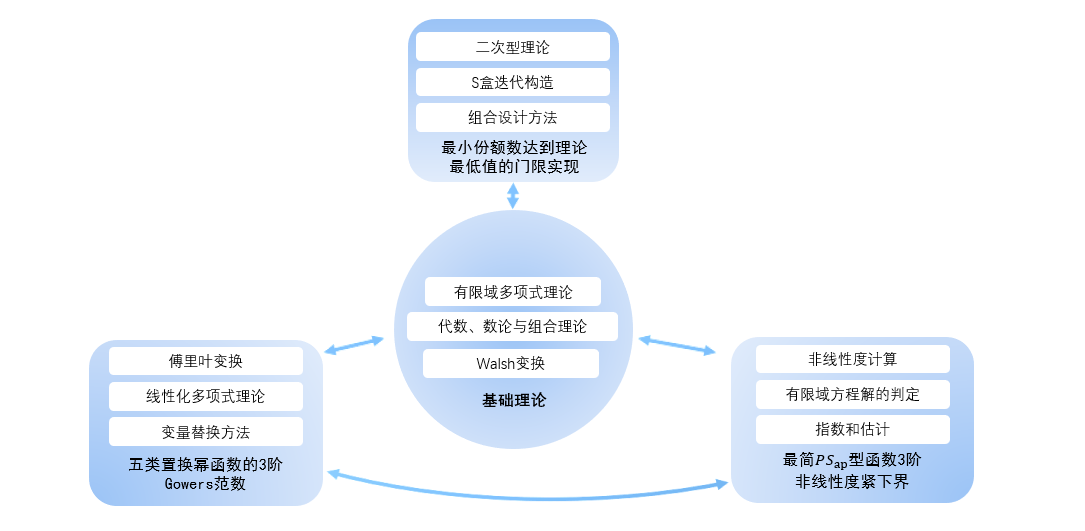
\includegraphics[width=17cm]{figures/Proposal_pic.png} 
    \caption{研究方案与技术路线框图}
    \label{pic:research_scheme}
\end{figure}
\subsection{研究方法与研究方案}
本课题的研究方法主要是首先掌握相关领域的国内外研究现状以及基本的研究方法和技巧,对其归纳总结并进行系统分析,以期在此基础上得到研究结果。
本课题研究方案与技术路线框图如图~\ref{pic:research_scheme} 所示。
下面我们结合研究内容和关键问题详细说明本课题的研究方法,我们的研究方案会针对两部分研究内容进行规划。
\subsubsection{低次逼近攻击中的密码学指标计算问题}
\begin{enumerate}[label=(\arabic{*})]
    \item 由于给出任意布尔函数的实际高阶非线性度是非常困难的,目前仅有一些变元个数很小的特殊布尔函数的实际二阶、三阶非线性度是已知的。
    对于变元个数较大的布尔函数,很难利用计算机计算其实际高阶非线性度,目前也没有有效的快速算法。
    因此我们拟利用函数的三阶非线性度的紧下界来衡量函数对低次逼近攻击的抵抗力。
    证明函数三阶非线性度的紧下界,在Carlet在文献~\cite{CC08IT}中提出的定理下,等价于确定该函数所有的二阶导函数的非线性度。
    根据Walsh谱计算公式,发现$\mathcal{PS}_{ap}$型函数二阶导的非线性度的计算与乘法逆函数的二阶差分方程的根有直接的关系,因此对乘法逆函数的二阶差分谱的理论证明帮助我们进一步梳理函数二阶导的非线性度的证明思路。
    在得到乘法逆函数的二阶差分谱结果后,确定函数二阶导非线性度问题,根据导数点的取值问题的求解方法可以分为两类。第一种情况是证明特定迹函数方程组有解,另一种情况是证明一类指数和的大小。
    我们可以通过迹函数的性质分析有限域上的迹函数方程组的解的数量是否不为零,从而确定对应非线性度大小。
    对一类指数和的精确计算是困难的,所以我们选择证明这类指数和的一个紧上界。结合代数曲线,通过计算曲线定义的曲面亏格大小,可以估计曲面的有理点的数量,同时根据曲线无穷远点的数量,可以证明这类指数和的一个紧上界,从而给出对应非线性度的一个紧下界。
    \item 即使是证明函数的高阶非线性度的一个紧下界都是具有一定挑战性的,因此我们拟利用其他密码学指标对函数抵抗低次逼近攻击的能力进行估计。
    根据国内外研究成果,利用函数Gowers范数的上界可以推导出函数的高阶非线性度的下界,因此本课题拟计算函数的Gowers范数,用于估计该函数的高阶非线性度。
    从向量布尔函数的Gowers范数定义出发,利用置换幂函数简单的数学结构,可以将$k$阶Gowers范数的计算等价为确定函数$k-1$阶差分谱。因此,研究五类能有效抵抗线性分析和差分分析的置换幂函数的Gowers范数,就是完全刻画这些函数的二阶差分谱。以证明Welch函数的$3$阶Gowers范数为例,证明的核心是计算函数的$2$阶差分谱,因为Welch函数代数次数为$3$,其$2$阶差分谱的计算本质上是计算一类线性的方程的根的数量。在本课题中,在变量替换方法下,问题的本质是计算一类线性的方程的落在一特定子空间上的根的数量。
    我们采用``squaring trick''方法处理方程,为显式地表达出方程的根提供可行性,从而推导方程的根落在要求的子空间上的充分必要条件,同时计算满足上述充要条件对应的根的数量,借此可以完全确定Welch函数二阶差分谱,从而确定该函数的$3$阶Gowers范数,因此估计了函数对二次逼近攻击的抵抗能力。
\end{enumerate}
\subsubsection{硬件实现代价低的门限实现方案}
在没有引入随机数的情况下,根据计算机搜索结果,大部分具有置换性质的非线性组件不存在份额数达到理论最低值的门限实现方案。
而门限实现的实现代价与所需的份额数的平方呈现正相关的关系,因此对份额数达到理论最低值的置换非线性组件亟待进一步探索。
对$n$元代数次数为$s$的置换函数构造份额数为$s+1$的门限实现方案实际上是构造具有特定性质的$n(s+1)$元代数次数为$s$的置换函数。
而函数为置换函数的充要条件是函数的所有分量函数均平衡,因此问题转化为确定所有分量函数是否平衡。
首先我们拟利用$n-1$元代数次数为$s-1$的置换函数,构造份额数为$s+1$的门限实现方案,也就是构造具有特定性质的$(n-1)(s+1)$元的置换函数。
故而问题集中在如何将$(n-1)(s+1)$元置换函数扩展为$(n+1)(s+1)$元置换函数,同时保证后者仍然具有特定性质。
由于二次函数结构简单,易于分析,本课题拟从$n$元二次置换函数出发,构造其份额数为$4$的门限实现方案,同时构造一个特殊的三次布尔函数,将二次置换函数扩充为三次置换函数。
又因为布尔函数份额数为理论最低值的门限实现是可行的,故主要研究在如何利用两个门限实现方案构造新的门限实现方案。
% 同时设计一个满足条件的$n(s+1)$元置换函数等价于构造一个$n$元布尔函数,并且该布尔函数做门限实现得到的$s+1$个函数,其线性组合后的结果与$(n-1)(s+1)$元的置换函数的任意分量函数之和都是平衡的。

\subsection{可行性分析}
整个研究方案的可行性在前人的工作中已经有了相当的基础,课题的进一步研究依赖于对现有方法更深入的拓展和创新。
前期的研究成果已经证明,量化函数对低次逼近攻击防护能力的相关工作是可实现的:
\begin{enumerate}[label=\arabic{*})]
    \item 在描述函数的低次逼近攻击的防护问题上,通常选择高阶非线性度或Gowers范数进行刻画。可以利用高阶非线性度的下界衡量函数对应密码学性质,其问题主要在于完全确定函数二阶差分谱和对部分指数和进行估计,而这些问题已经有比较成熟的求解思路,因此高阶非线性度的紧下界的理论推导是可行的。
    \item 当选择Gowers范数描述函数密码学性质时,置换幂函数的结构简单,理论成熟,因此利用置换幂函数的性质可以将问题简化为完全确定该函数的二阶差分谱。在函数次数为3的情况下,确定二阶差分谱等价于确定一类线性化的多项式的根。最后借助``squaring trick''或者其它有限域方法来处理线性化多项式,我们能够顺利地计算出对应的结果,从而确定二阶差分谱。
    \item 在设计一类非线性组件的门限实现方案过程中,利用``Direct Sharing''或者其他已知方法可以为代数次数为$t$的置换函数构造份额数为$t+2$的门限实现方案。通过分析二次函数的Dickson形式以及组合数学的结论,可以实现特殊条件的三次布尔函数的构造,因而最终构造一类门限实现方案份额数达到理论最低值的具有置换性质的非线性组件。
\end{enumerate}

\section{课题的创新点 Novelties of the proposed topic.}
本课题的主要创新点有以下几点:
\begin{enumerate}[label=(\arabic{*})]
    \item 首次证明了一类$\mathcal{PS}_{ap}$型函数的所有$2$阶导函数的非线性度或者非线性度的下界;
    \item 首次完全刻画了五类置换幂函数的二阶差分谱,并借此实现了函数3阶Gowers范数的计算;
    \item 构造一类非线性组件,其门限实现方案所需最小份额数达到理论最低$t+1$,且该组件非线性度不为零。
\end{enumerate}

\section{计划进度、预期成果 Research schedule, and expected outcomes.}
\begin{enumerate}[label=\arabic{*})]
    \item 文献资料检索阅读:2021 年 9 月至今
    \item 完成选题与开题报告:2022 年 7 月
    \item 研究关键问题,开展相关研究工作与论文撰写:2021 年 9 月至 2024 年 12 月
    \item 论文年度考核:学习期间每学年
    \item 论文撰写,印刷,答辩:时间待定
\end{enumerate}


\section{与本课题有关的工作积累、已有的研究工作成绩。
  Prior experience and accomplished achievements
  related to the proposed topic.}
\begin{enumerate}[label={[\arabic{*}]}]
    \item Li Z, Shen B, Tang D. A Lower Bound on the Third-order Nonlinearity of the Simplest $\mathcal{PS}_{ap}$ Bent Functions[J]. Discrete Applied Mathematics, 2024, 349: 148-161.
    \item Li Z, Tang D. The Gowers $U_3$ Norm of Five Classes of Power Permutations with Good Cryptographic Properties, Journal of Cryptography. (已投). 
\end{enumerate}



\vspace{\baselineskip}

% 剩下的所有内容均为仿宋加粗
\bfseries\fangsong
\noindent
本人承诺:开题报告中的内容真实无误,若有不实,愿承担相应的责任和后果。
I hereby declare and confirm that the details
provided in this Form are valid and accurate.
If anything untruthful found,
I will bear the corresponding liabilities and consequences.

\vspace{\baselineskip}

\noindent
学生签字/Signature of Student: 李兆乐
\hfill
日期/Date: 2024-05-DD

\end{document}